% Options for packages loaded elsewhere
\PassOptionsToPackage{unicode}{hyperref}
\PassOptionsToPackage{hyphens}{url}
%
\documentclass[
]{book}
\usepackage{amsmath,amssymb}
\usepackage{lmodern}
\usepackage{iftex}
\ifPDFTeX
  \usepackage[T1]{fontenc}
  \usepackage[utf8]{inputenc}
  \usepackage{textcomp} % provide euro and other symbols
\else % if luatex or xetex
  \usepackage{unicode-math}
  \defaultfontfeatures{Scale=MatchLowercase}
  \defaultfontfeatures[\rmfamily]{Ligatures=TeX,Scale=1}
\fi
% Use upquote if available, for straight quotes in verbatim environments
\IfFileExists{upquote.sty}{\usepackage{upquote}}{}
\IfFileExists{microtype.sty}{% use microtype if available
  \usepackage[]{microtype}
  \UseMicrotypeSet[protrusion]{basicmath} % disable protrusion for tt fonts
}{}
\makeatletter
\@ifundefined{KOMAClassName}{% if non-KOMA class
  \IfFileExists{parskip.sty}{%
    \usepackage{parskip}
  }{% else
    \setlength{\parindent}{0pt}
    \setlength{\parskip}{6pt plus 2pt minus 1pt}}
}{% if KOMA class
  \KOMAoptions{parskip=half}}
\makeatother
\usepackage{xcolor}
\IfFileExists{xurl.sty}{\usepackage{xurl}}{} % add URL line breaks if available
\IfFileExists{bookmark.sty}{\usepackage{bookmark}}{\usepackage{hyperref}}
\hypersetup{
  pdftitle={Sonorezé},
  pdfauthor={Tristan Lorino},
  hidelinks,
  pdfcreator={LaTeX via pandoc}}
\urlstyle{same} % disable monospaced font for URLs
\usepackage{color}
\usepackage{fancyvrb}
\newcommand{\VerbBar}{|}
\newcommand{\VERB}{\Verb[commandchars=\\\{\}]}
\DefineVerbatimEnvironment{Highlighting}{Verbatim}{commandchars=\\\{\}}
% Add ',fontsize=\small' for more characters per line
\usepackage{framed}
\definecolor{shadecolor}{RGB}{248,248,248}
\newenvironment{Shaded}{\begin{snugshade}}{\end{snugshade}}
\newcommand{\AlertTok}[1]{\textcolor[rgb]{0.94,0.16,0.16}{#1}}
\newcommand{\AnnotationTok}[1]{\textcolor[rgb]{0.56,0.35,0.01}{\textbf{\textit{#1}}}}
\newcommand{\AttributeTok}[1]{\textcolor[rgb]{0.77,0.63,0.00}{#1}}
\newcommand{\BaseNTok}[1]{\textcolor[rgb]{0.00,0.00,0.81}{#1}}
\newcommand{\BuiltInTok}[1]{#1}
\newcommand{\CharTok}[1]{\textcolor[rgb]{0.31,0.60,0.02}{#1}}
\newcommand{\CommentTok}[1]{\textcolor[rgb]{0.56,0.35,0.01}{\textit{#1}}}
\newcommand{\CommentVarTok}[1]{\textcolor[rgb]{0.56,0.35,0.01}{\textbf{\textit{#1}}}}
\newcommand{\ConstantTok}[1]{\textcolor[rgb]{0.00,0.00,0.00}{#1}}
\newcommand{\ControlFlowTok}[1]{\textcolor[rgb]{0.13,0.29,0.53}{\textbf{#1}}}
\newcommand{\DataTypeTok}[1]{\textcolor[rgb]{0.13,0.29,0.53}{#1}}
\newcommand{\DecValTok}[1]{\textcolor[rgb]{0.00,0.00,0.81}{#1}}
\newcommand{\DocumentationTok}[1]{\textcolor[rgb]{0.56,0.35,0.01}{\textbf{\textit{#1}}}}
\newcommand{\ErrorTok}[1]{\textcolor[rgb]{0.64,0.00,0.00}{\textbf{#1}}}
\newcommand{\ExtensionTok}[1]{#1}
\newcommand{\FloatTok}[1]{\textcolor[rgb]{0.00,0.00,0.81}{#1}}
\newcommand{\FunctionTok}[1]{\textcolor[rgb]{0.00,0.00,0.00}{#1}}
\newcommand{\ImportTok}[1]{#1}
\newcommand{\InformationTok}[1]{\textcolor[rgb]{0.56,0.35,0.01}{\textbf{\textit{#1}}}}
\newcommand{\KeywordTok}[1]{\textcolor[rgb]{0.13,0.29,0.53}{\textbf{#1}}}
\newcommand{\NormalTok}[1]{#1}
\newcommand{\OperatorTok}[1]{\textcolor[rgb]{0.81,0.36,0.00}{\textbf{#1}}}
\newcommand{\OtherTok}[1]{\textcolor[rgb]{0.56,0.35,0.01}{#1}}
\newcommand{\PreprocessorTok}[1]{\textcolor[rgb]{0.56,0.35,0.01}{\textit{#1}}}
\newcommand{\RegionMarkerTok}[1]{#1}
\newcommand{\SpecialCharTok}[1]{\textcolor[rgb]{0.00,0.00,0.00}{#1}}
\newcommand{\SpecialStringTok}[1]{\textcolor[rgb]{0.31,0.60,0.02}{#1}}
\newcommand{\StringTok}[1]{\textcolor[rgb]{0.31,0.60,0.02}{#1}}
\newcommand{\VariableTok}[1]{\textcolor[rgb]{0.00,0.00,0.00}{#1}}
\newcommand{\VerbatimStringTok}[1]{\textcolor[rgb]{0.31,0.60,0.02}{#1}}
\newcommand{\WarningTok}[1]{\textcolor[rgb]{0.56,0.35,0.01}{\textbf{\textit{#1}}}}
\usepackage{longtable,booktabs,array}
\usepackage{calc} % for calculating minipage widths
% Correct order of tables after \paragraph or \subparagraph
\usepackage{etoolbox}
\makeatletter
\patchcmd\longtable{\par}{\if@noskipsec\mbox{}\fi\par}{}{}
\makeatother
% Allow footnotes in longtable head/foot
\IfFileExists{footnotehyper.sty}{\usepackage{footnotehyper}}{\usepackage{footnote}}
\makesavenoteenv{longtable}
\usepackage{graphicx}
\makeatletter
\def\maxwidth{\ifdim\Gin@nat@width>\linewidth\linewidth\else\Gin@nat@width\fi}
\def\maxheight{\ifdim\Gin@nat@height>\textheight\textheight\else\Gin@nat@height\fi}
\makeatother
% Scale images if necessary, so that they will not overflow the page
% margins by default, and it is still possible to overwrite the defaults
% using explicit options in \includegraphics[width, height, ...]{}
\setkeys{Gin}{width=\maxwidth,height=\maxheight,keepaspectratio}
% Set default figure placement to htbp
\makeatletter
\def\fps@figure{htbp}
\makeatother
\setlength{\emergencystretch}{3em} % prevent overfull lines
\providecommand{\tightlist}{%
  \setlength{\itemsep}{0pt}\setlength{\parskip}{0pt}}
\setcounter{secnumdepth}{5}
\usepackage{booktabs}
\usepackage{amsthm}
\makeatletter
\def\thm@space@setup{%
  \thm@preskip=8pt plus 2pt minus 4pt
  \thm@postskip=\thm@preskip
}
\makeatother
\ifLuaTeX
  \usepackage{selnolig}  % disable illegal ligatures
\fi
\usepackage[]{natbib}
\bibliographystyle{apalike}

\title{Sonorezé}
\author{Tristan Lorino}
\date{2022-05-10}

\begin{document}
\maketitle

{
\setcounter{tocdepth}{1}
\tableofcontents
}
\hypertarget{pruxe9sentation}{%
\chapter{Présentation}\label{pruxe9sentation}}

\hypertarget{configuration}{%
\section{Configuration}\label{configuration}}

\hypertarget{configuration-de-knitr}{%
\section{\texorpdfstring{Configuration de \emph{knitr}}{Configuration de knitr}}\label{configuration-de-knitr}}

Pour afficher par défaut les morceaux de code R (\textbf{chunks}) :

\begin{Shaded}
\begin{Highlighting}[]
\NormalTok{knitr}\SpecialCharTok{::}\NormalTok{opts\_chunk}\SpecialCharTok{$}\FunctionTok{set}\NormalTok{(}\AttributeTok{echo =} \ConstantTok{TRUE}\NormalTok{)}
\end{Highlighting}
\end{Shaded}

Pour que \textbf{knitr} retrouve tous ses (nos) petits :

\begin{Shaded}
\begin{Highlighting}[]
\NormalTok{knitr}\SpecialCharTok{::}\NormalTok{opts\_knit}\SpecialCharTok{$}\FunctionTok{set}\NormalTok{(}\AttributeTok{root.dir =}\NormalTok{ rprojroot}\SpecialCharTok{::}\FunctionTok{find\_rstudio\_root\_file}\NormalTok{())}
\end{Highlighting}
\end{Shaded}

Par défaut on n'utilise pas de cache :

\begin{Shaded}
\begin{Highlighting}[]
\NormalTok{knitr}\SpecialCharTok{::}\NormalTok{opts\_chunk}\SpecialCharTok{$}\FunctionTok{set}\NormalTok{(}\AttributeTok{cache =}\ConstantTok{FALSE}\NormalTok{)}
\end{Highlighting}
\end{Shaded}

Pour la typo française, on précise que les décimales seront séparées des entiers par une virgule :

\begin{Shaded}
\begin{Highlighting}[]
\FunctionTok{options}\NormalTok{(}\AttributeTok{OutDec=}\StringTok{","}\NormalTok{)}
\end{Highlighting}
\end{Shaded}

Pour les sorties francisées (par exemple les noms des mois) :

\begin{Shaded}
\begin{Highlighting}[]
\FunctionTok{Sys.setlocale}\NormalTok{(}\StringTok{"LC\_CTYPE"}\NormalTok{,}\StringTok{"fr\_FR.UTF{-}8"}\NormalTok{)}
\end{Highlighting}
\end{Shaded}

\hypertarget{duxe9ploiement-sur-github-pages}{%
\section{Déploiement sur GitHub Pages}\label{duxe9ploiement-sur-github-pages}}

GitHub Pages va puiser les pages html dans le dossier \textbf{/docs}. Pour déployer le \emph{bookdown} sur Github, on ajoute au fichier \_bookdown.yml la commande :

\begin{Shaded}
\begin{Highlighting}[]
\NormalTok{output\_dir}\SpecialCharTok{:} \StringTok{"docs"}
\end{Highlighting}
\end{Shaded}

Remember each Rmd file contains one and only one chapter, and a chapter is defined by the first-level heading \texttt{\#}.

\begin{verbatim}
## Le chargement a nécessité le package : pacman
\end{verbatim}

On charge les données issues de \emph{metabase} et on indique le dossier de travail :

\begin{Shaded}
\begin{Highlighting}[]
\FunctionTok{load}\NormalTok{(}\FunctionTok{here}\NormalTok{(}\StringTok{"noisecapture\_data.Rda"}\NormalTok{))}
\FunctionTok{here}\NormalTok{()}
\end{Highlighting}
\end{Shaded}

\begin{verbatim}
## [1] "/Users/tristanlorino/Documents/GitHub/WorkinprogReze"
\end{verbatim}

\begin{Shaded}
\begin{Highlighting}[]
\FunctionTok{source}\NormalTok{(}\FunctionTok{here}\NormalTok{(}\StringTok{"R"}\NormalTok{,}\StringTok{"Statistiques.R"}\NormalTok{))}
\CommentTok{\#source("./Users/tristanlorino/Documents/GitHub/WorkinprogReze/docs/Statistiques.R")}

\NormalTok{noisecapture\_data }\OtherTok{\textless{}{-}} \FunctionTok{as.data.frame}\NormalTok{(noisecapture\_data)}
\NormalTok{trace\_table }\OtherTok{\textless{}{-}} \FunctionTok{as.data.frame}\NormalTok{(noisecapture\_data[,}\FunctionTok{c}\NormalTok{(}\StringTok{"Id"}\NormalTok{,}\StringTok{"Date"}\NormalTok{,}\StringTok{"x"}\NormalTok{,}\StringTok{"y"}\NormalTok{,}\StringTok{"leq\_mean"}\NormalTok{,}\StringTok{"tags"}\NormalTok{)]) }\SpecialCharTok{\%\textgreater{}\%}
  \FunctionTok{arrange}\NormalTok{(Id,Date) }\SpecialCharTok{\%\textgreater{}\%}
  \FunctionTok{group\_by}\NormalTok{(Id) }\SpecialCharTok{\%\textgreater{}\%}
  \FunctionTok{arrange}\NormalTok{(Date) }\SpecialCharTok{\%\textgreater{}\%}
  \FunctionTok{mutate}\NormalTok{(}\AttributeTok{IdTraceReset=}\FunctionTok{cumsum}\NormalTok{(}\FunctionTok{c}\NormalTok{(}\ConstantTok{TRUE}\NormalTok{, }\FunctionTok{as.integer}\NormalTok{(}\FunctionTok{diff}\NormalTok{(}\FunctionTok{as.POSIXct}\NormalTok{(Date)), }\AttributeTok{units =} \StringTok{"secs"}\NormalTok{) }\SpecialCharTok{\textgreater{}=}\NormalTok{ 2L))) }\SpecialCharTok{\%\textgreater{}\%}
  \FunctionTok{ungroup}\NormalTok{() }\SpecialCharTok{\%\textgreater{}\%}
  \FunctionTok{mutate}\NormalTok{(}\AttributeTok{IdGlobal=}\FunctionTok{str\_c}\NormalTok{(Id,IdTraceReset)) }\SpecialCharTok{\%\textgreater{}\%}
  \FunctionTok{arrange}\NormalTok{(IdGlobal) }\SpecialCharTok{\%\textgreater{}\%}
  \FunctionTok{group\_by}\NormalTok{(Id) }\SpecialCharTok{\%\textgreater{}\%}
  \FunctionTok{arrange}\NormalTok{(IdTraceReset) }\SpecialCharTok{\%\textgreater{}\%}
  \FunctionTok{group\_by}\NormalTok{(IdGlobal) }\SpecialCharTok{\%\textgreater{}\%}
  \FunctionTok{mutate}\NormalTok{(}\AttributeTok{IdTrace=}\FunctionTok{cur\_group\_id}\NormalTok{()) }\SpecialCharTok{\%\textgreater{}\%}
  \FunctionTok{ungroup}\NormalTok{() }\SpecialCharTok{\%\textgreater{}\%}
  \FunctionTok{distinct}\NormalTok{(IdTrace, }\AttributeTok{.keep\_all =} \ConstantTok{TRUE}\NormalTok{)}

\NormalTok{tags\_table }\OtherTok{\textless{}{-}}\NormalTok{ trace\_table }\SpecialCharTok{\%\textgreater{}\%}
  \FunctionTok{filter}\NormalTok{(tags }\SpecialCharTok{!=} \StringTok{""}\NormalTok{) }\SpecialCharTok{\%\textgreater{}\%}
  \FunctionTok{filter}\NormalTok{(x }\SpecialCharTok{!=} \StringTok{"NA"}\NormalTok{) }\SpecialCharTok{\%\textgreater{}\%}
  \FunctionTok{select}\NormalTok{(}\SpecialCharTok{{-}}\FunctionTok{c}\NormalTok{(IdGlobal,IdTraceReset))}
\end{Highlighting}
\end{Shaded}

La procédure consiste à :

\begin{itemize}
\tightlist
\item
  créer un identifiant par trace (suite d'enregistrements successifs) ;
\item
  ne garder qu'un enregistrement par trace ;
\item
  supprimer les traces qui n'ont pas été taggées, ainsi que celles sans coordonnées GPS :
\end{itemize}

\begin{verbatim}
## # A tibble: 10 x 7
##    Id    Date                    x     y leq_mean tags                   IdTrace
##    <chr> <dttm>              <dbl> <dbl>    <dbl> <chr>                    <int>
##  1 029d  2021-12-06 22:54:28 -1.56  47.2     42.0 indoor                       1
##  2 045d  2022-01-19 14:33:40 -1.57  47.2     51.1 test,chatting,footste~       7
##  3 10fe  2022-01-14 11:06:50 -1.56  47.2     55.3 indoor,chatting             15
##  4 184d  2022-01-13 16:21:59 -1.54  47.2     69.4 test,chatting,childre~      21
##  5 284c  2022-03-17 15:10:37 -1.53  47.2     70.3 road                        22
##  6 29f2  2021-12-07 17:33:00 -1.56  47.2     44.1 indoor                      25
##  7 2d6c  2021-12-07 08:53:59 -1.58  47.2     58.7 road,animals                44
##  8 2dad  2022-03-04 10:06:30 -1.58  47.2     56.3 road                        48
##  9 2f32  2021-12-01 19:21:35 -1.56  47.2     77.9 test,indoor                 49
## 10 32cc  2021-11-27 21:24:14 -1.54  47.2     66.2 indoor,footsteps            59
\end{verbatim}

\begin{itemize}
\tightlist
\item
  à partir de la colonne «~tags~», qui contient pour chaque trace (chaque ligne) un ou plusieurs tags séparés par des virgules : créer une nouvelle colonne «~tags~» avec un seul tag (par ligne), quitte à dupliquer une trace (une ligne) lorsque cette-dernière a plusieurs tags :
\end{itemize}

\begin{verbatim}
## # A tibble: 10 x 8
##    Id    Date                    x     y leq_mean tags       IdTrace TagGroup 
##    <chr> <dttm>              <dbl> <dbl>    <dbl> <chr>        <int> <chr>    
##  1 029d  2021-12-06 22:54:28 -1.56  47.2     42.0 indoor           1 Condition
##  2 045d  2022-01-19 14:33:40 -1.57  47.2     51.1 test             7 Condition
##  3 045d  2022-01-19 14:33:40 -1.57  47.2     51.1 chatting         7 Ambiance 
##  4 045d  2022-01-19 14:33:40 -1.57  47.2     51.1 footsteps        7 Ambiance 
##  5 045d  2022-01-19 14:33:40 -1.57  47.2     51.1 water            7 Ambiance 
##  6 045d  2022-01-19 14:33:40 -1.57  47.2     51.1 animals          7 Ambiance 
##  7 045d  2022-01-19 14:33:40 -1.57  47.2     51.1 vegetation       7 Ambiance 
##  8 045d  2022-01-19 14:33:40 -1.57  47.2     51.1 works            7 Ambiance 
##  9 10fe  2022-01-14 11:06:50 -1.56  47.2     55.3 indoor          15 Condition
## 10 10fe  2022-01-14 11:06:50 -1.56  47.2     55.3 chatting        15 Ambiance
\end{verbatim}

\hypertarget{intro}{%
\chapter{Introduction}\label{intro}}

You can label chapter and section titles using \texttt{\{\#label\}} after them, e.g., we can reference Chapter \ref{intro}. If you do not manually label them, there will be automatic labels anyway, e.g., Chapter \ref{methods}.

Figures and tables with captions will be placed in \texttt{figure} and \texttt{table} environments, respectively.

\begin{Shaded}
\begin{Highlighting}[]
\FunctionTok{par}\NormalTok{(}\AttributeTok{mar =} \FunctionTok{c}\NormalTok{(}\DecValTok{4}\NormalTok{, }\DecValTok{4}\NormalTok{, .}\DecValTok{1}\NormalTok{, .}\DecValTok{1}\NormalTok{))}
\FunctionTok{plot}\NormalTok{(pressure, }\AttributeTok{type =} \StringTok{\textquotesingle{}b\textquotesingle{}}\NormalTok{, }\AttributeTok{pch =} \DecValTok{19}\NormalTok{)}
\end{Highlighting}
\end{Shaded}

\begin{figure}

{\centering 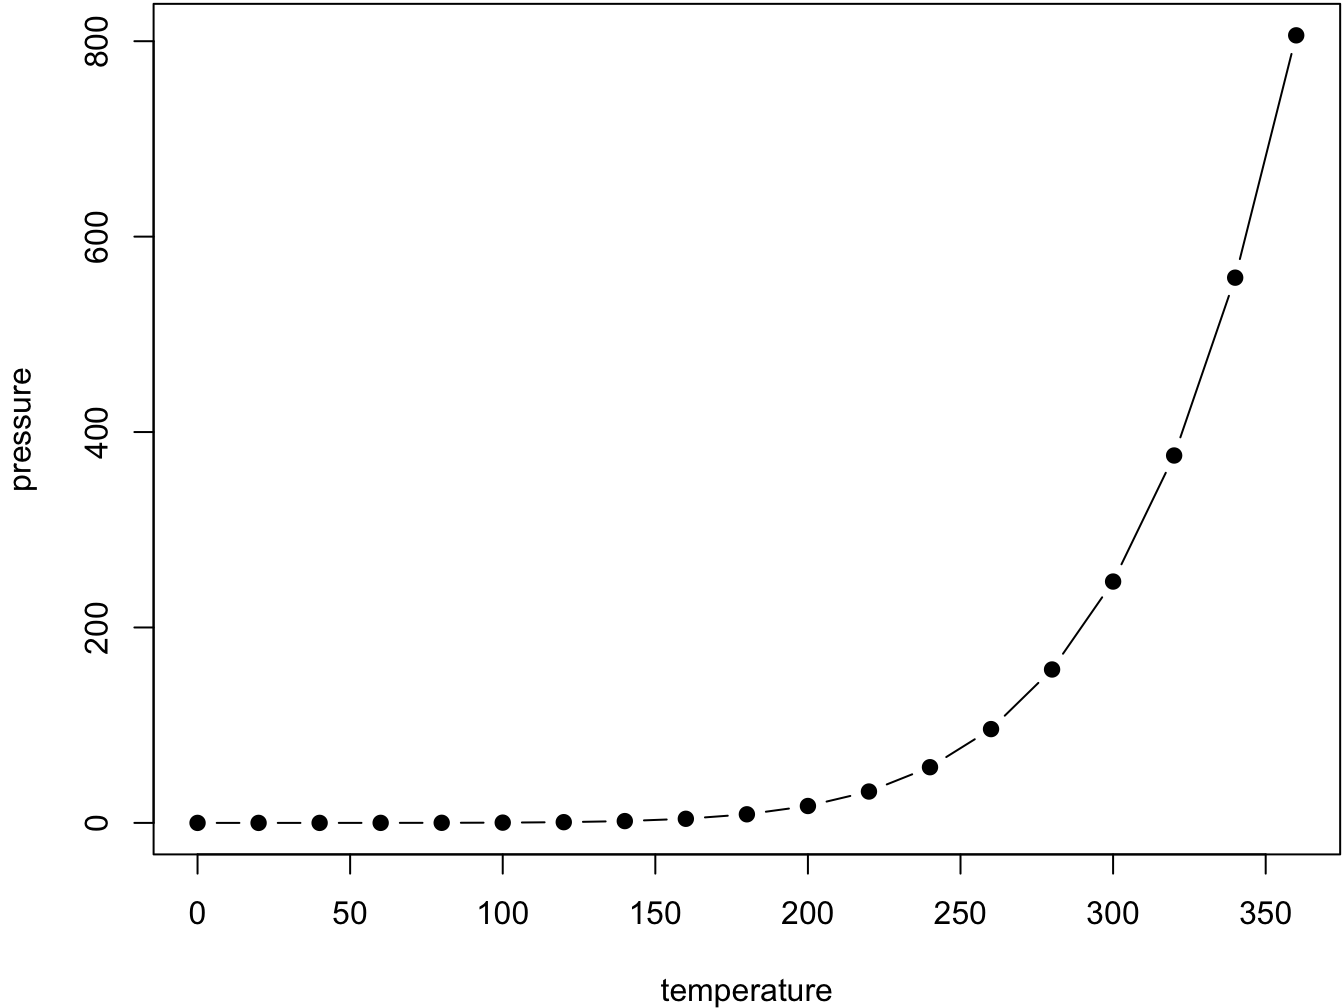
\includegraphics[width=0.8\linewidth]{bookdown-demo_files/figure-latex/nice-fig-1} 

}

\caption{Here is a nice figure!}\label{fig:nice-fig}
\end{figure}

Reference a figure by its code chunk label with the \texttt{fig:} prefix, e.g., see Figure \ref{fig:nice-fig}. Similarly, you can reference tables generated from \texttt{knitr::kable()}, e.g., see Table \ref{tab:nice-tab}.

\begin{Shaded}
\begin{Highlighting}[]
\NormalTok{knitr}\SpecialCharTok{::}\FunctionTok{kable}\NormalTok{(}
  \FunctionTok{head}\NormalTok{(iris, }\DecValTok{20}\NormalTok{), }\AttributeTok{caption =} \StringTok{\textquotesingle{}Here is a nice table!\textquotesingle{}}\NormalTok{,}
  \AttributeTok{booktabs =} \ConstantTok{TRUE}
\NormalTok{)}
\end{Highlighting}
\end{Shaded}

\begin{table}

\caption{\label{tab:nice-tab}Here is a nice table!}
\centering
\begin{tabular}[t]{rrrrl}
\toprule
Sepal.Length & Sepal.Width & Petal.Length & Petal.Width & Species\\
\midrule
5,1 & 3,5 & 1,4 & 0,2 & setosa\\
4,9 & 3,0 & 1,4 & 0,2 & setosa\\
4,7 & 3,2 & 1,3 & 0,2 & setosa\\
4,6 & 3,1 & 1,5 & 0,2 & setosa\\
5,0 & 3,6 & 1,4 & 0,2 & setosa\\
\addlinespace
5,4 & 3,9 & 1,7 & 0,4 & setosa\\
4,6 & 3,4 & 1,4 & 0,3 & setosa\\
5,0 & 3,4 & 1,5 & 0,2 & setosa\\
4,4 & 2,9 & 1,4 & 0,2 & setosa\\
4,9 & 3,1 & 1,5 & 0,1 & setosa\\
\addlinespace
5,4 & 3,7 & 1,5 & 0,2 & setosa\\
4,8 & 3,4 & 1,6 & 0,2 & setosa\\
4,8 & 3,0 & 1,4 & 0,1 & setosa\\
4,3 & 3,0 & 1,1 & 0,1 & setosa\\
5,8 & 4,0 & 1,2 & 0,2 & setosa\\
\addlinespace
5,7 & 4,4 & 1,5 & 0,4 & setosa\\
5,4 & 3,9 & 1,3 & 0,4 & setosa\\
5,1 & 3,5 & 1,4 & 0,3 & setosa\\
5,7 & 3,8 & 1,7 & 0,3 & setosa\\
5,1 & 3,8 & 1,5 & 0,3 & setosa\\
\bottomrule
\end{tabular}
\end{table}

You can write citations, too. For example, we are using the \textbf{bookdown} package \citep{R-bookdown} in this sample book, which was built on top of R Markdown and \textbf{knitr} \citep{xie2015}.

\hypertarget{literature}{%
\chapter{Literature}\label{literature}}

Here is a review of existing methods.

  \bibliography{book.bib,packages.bib}

\end{document}
